\documentclass[10pt, a4paper]{article}
\title{\textbf{{\Huge 프리드버그 선형대수학 요약본}}}
\author{Lee Jhun Hyeok\,(wnsx0000@gmail.com)}
\date{\today}

\usepackage{graphicx} % Required for inserting images
\usepackage{kotex}
\usepackage{geometry}
\usepackage{parskip}
\usepackage{amsthm}
\usepackage{amsmath}

\usepackage{tikz}
\usetikzlibrary{positioning}

\geometry{
 a4paper,
 left=25mm,
 right=25mm,
 top=30mm,
 bottom=30mm
 }
 \hbadness=199999  % or any number >=10000, 임시로 사용

\begin{document}
% 제목
\maketitle

% 목차
\textbf{\textit{목차}}

\textbf{\textit{Part 1. 벡터공간\\}}
1. 벡터공간\\
2. 부분공간\\
3. 일차결합과 연립일차방정식\\
4. 일차종속과 일차독립\\
5. 기저와 차원

\textbf{\textit{Part 2. 선형변환과 행렬\\}}
1. 선형변환\\
2. 선형변환의 행렬표현\\
3. 선형변환의 합성과 행렬 곱\\
4. 가역성과 동형사상\\
5. 좌표변환 행렬

\newpage

% 내용
%1.벡터공간\part{\textit{\underline{벡터공간}}}
\part*{1. 벡터공간}

\section*{1. 벡터공간(vector space)}

\subsubsection*{1) 정의}

체 $F$에서의 벡터공간(vector space) 또는 선형공간(linear space) $V$는 다음 8가지 조건을 만족시키는 두 연산, 합과 스칼라 곱을 가지는 집합임.

\begin{itemize}
\item 합(sum)은 $V$의 두 원소 $x, y$에 대하여 유일한 원소 $x+y \in V$를 대응하는 연산임.
\item 스칼라 곱(scalar multiplication)은 체 $F$의 원소 $a$와 벡터공간 $V$의 원소 $x$마다 유일한 원소 $ax \in V$를 대응하는 연산이다. 이때 $ax$는 $a$와 $x$의 스칼라 곱(product)이라 함.
\end{itemize}

(VS1) 모든 $x,y \in V$에 대하여 $x+y=y+x$임. (덧셈의 교환법칙)\\
(VS2) 모든 $x,y,z \in V$에 대하여 $(x+y)+z=x+(y+z)$임. (덧셈의 결합법칙)\\
(VS3) 모든 $x \in V$에 대하여 $x+0=x$인 $0 \in V$가 존재함. (덧셈에 대한 항등원, 즉 영벡터 존재)\\
(VS4) 각 $x \in V$마다 $x+y=0$인 $y \in V$가 존재함. (덧셈에 대한 역원, 즉 역벡터 존재)\\
(VS5) 각 $x \in V$에 대하여 $1x=x$임. (스칼라 곱에 대한 항등원 존재)\\
(VS6) 모든 $a,b \in F$와 모든 $x \in V$에 대하여 $(ab)x=a(bx)$임.\\
(VS7) 모든 $a \in F$와 모든 $x,y \in V$에 대하여 $a(x+y)=ax+ay$임.\\
(VS8) 모든 $a,b \in F$와 모든 $x \in V$에 대하여 $(a+b)x=ax+bx$임.

\subsubsection*{2) 벡터공간의 표기}
체 $F$에서의 벡터공간 $V$는 $F-$벡터공간 $V$라고 표기함.

혼동의 여지가 없는 경우 체 $F$는 생략하기도 함.

\subsubsection*{3) 벡터와 스칼라}
벡터공간 $V$의 원소를 벡터, 체 $F$의 원소를 스칼라라 함.

여기서의 벡터는 벡터공간의 원소를 가리키는 일반적인 개념임.\\
지금까지 단순 화살표로 표현해 온 벡터를 포괄하는 의미.

(VS3)을 만족하는 유일한 벡터 $0$은 $V$의 영백터(zero vector)라 함.

(VS4)를 만족하는 유일한 벡터 $y$($-x$)는 덧셈에 대한 $x$의 역벡터(additive inverse)라고 함.


\newpage


\section*{2. 관련 정리}
\subsubsection*{1) 벡터 합의 소거법칙}
\textbf{Theorem 1.1}\, $x,y,z \in V$이고 $x+z=y+z$ 일 때, $x = y$ 임.

\textbf{Corollary 1}\, (VS3)을 만족하는 벡터 $0$(영백터)은 유일함.

\textbf{Corollary 2}\, (VS4)를 만족하는 벡터 $y$(역벡터)는 유일함.

\subsubsection*{2) 스칼라 곱 관련 성질\footnote{스칼라, 벡터, 영벡터 사이의 곱에 대한 정리.}}

\textbf{Theorem 1.2}\, 모든 벡터공간 $V$에 대해서 다음이 성립함.

\begin{enumerate}
    \item 모든 벡터 $x$에 대하여 $0x= \vec{0}$임.
    \item 모든 스칼라 $a$와 모든 벡터 $x$에 대하여 $(-a)x=-(ax)=a(-x)$임.
    \item 모든 스칼라 $a$에 대하여 $a \vec{0} = \vec{0}$임.\\
\end{enumerate}



\section*{3. 벡터공간의 예시\footnote{아래의 예시들은 각 성분별로(component-wise) 계산이 가능하기 때문에 매번 8가지 조건들을 검토할 필요가 없음.}}
\subsubsection*{1) $n$순서쌍(n-tuple)의 집합($F^n$)}
체 $F$에서 성분을 가져온 $n$순서쌍의 집합을 $F^n$이라 표기함.

$u=(a_1,a_2, ... ,a_n) \in F^n$, $v=(b_1,b_2, ... ,b_n) \in F^n$, $c \in F$ 일 때, 합과 스칼라 곱을 아래와 같이 정의하면 이 집합은 $F$-벡터공간임.

\[u+v=(a_1+b_1,a_2+b_2, ... ,a_n+b_n),\,cu=(ca_1,ca_2, ... ,ca_n)\]

$F^n$의 벡터는 행벡터(row vector)보다 열벡터(column vector)로 주로 표현함.

$F^1$은 그냥 $F$로 표현하는 경우가 많음.


\subsubsection*{2) 행렬(matrix)의 집합($M_{m \times n}(F)$)}
성분이 체 $F$의 원소인 모든 $m \times n$ 행렬의 집합은 $M_{m \times n}(F)$라 정의함.

$A,B \in M_{m \times n}(F)$, $c \in F$ 일 때, 합과 스칼라 곱을 아래와 같이 정의하면 이 집합은 $F$-벡터공간임.

\[(A+B)_{ij}=A_{ij}+B_{ij},\,(cA)_{ij}=cA_{ij}\]


\subsubsection*{3) 함수(function)의 집합($\mathcal{F}(S,F)$)}
체 $F$의 공집합이 아닌 부분집합 $S$가 있을 때, $\mathcal{F}(S,F)$는 $S$에서 $F$로 가는 모든 함수의 집합임.

$\mathcal{F}(S,F)$에서 모든 $s \in S$에 대하여 $f(s)=g(s)$일 때, 두 함수 $f$, $g$는 같다고 함.

$f,g \in \mathcal{F}(S,F)$, $c \in F$, $s \in S$ 일 때, 합과 스칼라 곱을 아래와 같이 정의하면 이 집합은 $F$-벡터공간임.

\[(f+g)(s)=f(s)+g(s),\,(cf)(s)=c(f(s))\]

실수집합 $R$에서 $R$로 가는 모든 연속함수의 집합을 $C(R)$이라 함.\\


\subsubsection*{4) 다항식(polynominal)의 집합($P(F)$)}
체 $F$에서 계수를 가져온 모든 다항식의 집합을 $P(F)$라 함.

두 다항식의 합과 스칼라 곱을 아래와 같이 정의하면 이 집합은 $F$-벡터공간임.

\[f(x)+g(x)=(a_n+b_n)x_n+(a_{n-1}+b_{n-1})x^{n-1}+ \cdots +(a_1+b_1)x+(a_0+b_0)\]
\[cf(x)=ca_nx_n+ca_{n-1}x^{n-1}+ \cdots +ca_1x+ca_0\]

음이 아닌 정수 $n$에 대하여 $P_n(F)$는 $n$ 이하의 차수를 가진 다항식의 집합임.


\subsubsection*{5) 수열의 집합}
체 $F$에서 정의된 모든 수열의 집합을 $V$라 할 때, $t \in F$와 두 수열 $(a_n)$, $(b_n)$에 대해서 합과 스칼라 곱을 정의하면 이 집합은 $F$-벡터공간임.

\[(a_n)+(b_n)=(a_n+b_n),\,t(a_n)=(ta_n)\]\\


\newpage


\part*{2. 부분공간(subspace)}

\section*{1. 부분공간\footnote{부분공간은 벡터공간의 일부분을 살펴보기 위해 존재한다고 이해하자.}}
\subsubsection*{1) 정의}
$F$-벡터공간 $V$의 부분집합 $W$가 $V$에서 정의한 합과 스칼라 곱을 가진 $F$-벡터공간일 때, $W$를 $V$의 부분공간이라 함.

즉, 벡터공간인 부모의 연산을 그대로 물려받은 벡터공간인 부분집합.

모든 벡터공간 $V$에 대하여 $V$와 $\{ 0 \}$은 $V$의 부분공간임.\\
특히 ${0}$는 점공간인 부분공간(zero subspace)이라고 함.

\subsubsection*{2) 부분공간 판별}
어떤 부분집합이 부분공간이기 위한 필요충분조건은 아래 4가지 성질을 만족하는 것임.\\
벡터공간의 8가지 조건을 생각해 보면 당연한 이야기.

\begin{enumerate}
    \item 모든 $x \in W$, $y \in W$에 대하여 $x+y \in W$임. ($W$는 합에 대하여 닫혀 있음)
    \item 모든 $c \in F$와 모든 $x \in W$에 대하여 $cx \in W$임. ($W$는 스칼라 곱에 대하여 닫혀 있음)
    \item $W$는 영벡터를 포함함. (영벡터 존재)
    \item $W$에 속한 모든 벡터 각각의 덧셈에 대한 역벡터는 $W$의 원소임. (역벡터 존재)
\end{enumerate}

Theorem 1.3에 따르면 $W$와 $V$의 영벡터는 반드시 같고, 4번 성질은 굳이 확인할 필요가 없음(항상 성립)\\


\section*{2. 관련 정리}
\subsubsection*{1) 부분공간 판별}
\textbf{Theorem 1.3}\, 벡터공간 $V$와 그 부분집합 $W$에 대하여, $W$가 $V$의 부분공간이기 위한 필요충분조건은 아래의 세 가지 조건을 만족하는 것임.

\begin{enumerate}
    \item $0 \in W$
    \item 모든 $x \in W$, $y \in W$에 대하여 $x+y \in W$
    \item 모든 $c \in F$와 모든 $x \in W$에 대하여 $cx \in W$
\end{enumerate}

\subsubsection*{2) 부분공간의 교집합}

\textbf{Theorem 1.4}\, 벡터공간 $V$의 부분공간들의 임의의 교집합은 $V$의 부분공간임.\\


\newpage


\part*{3. 일차결합과 연립일차방정식}

\section*{1. 일차결합(linear combination)}

\subsubsection*{1) 정의}
벡터공간 $V$의 공집합이 아닌 부분집합 $S$가 있다고 하자. 유한개의 벡터 $u_1,u_2, \cdots ,u_n \in S$와 스칼라 $a_1,a_2, \cdots , a_n$에 대하여 아래를 만족하는 벡터 $v \in V$를 $S$의 일차결합이라 함.

\[v=a_1u_1+a_2u_2+ \cdots +a_nu_n\]

이때, $v$는 벡터 $u_1,u_2, \cdots , u_n$의 일차결합이라 하고, $a_1,a_2, \cdots , a_n$은 이 일차결합의 계수(coefficient)라고 함.

영벡터는 공집합이 아닌 모든 부분집합의 일차결합임.\\


\section*{2. 연립일차방정식}
\subsubsection*{1) 일차결합과 연립일차방정식}
어떤 벡터가 일차결합으로 표현될 수 있는지를 연립일차방정식의 해를 구해 알아낼 수 있음.

어떤 벡터가 일차결합으로 표현될 수 있는지는 연립일차방정식의 풀이와 관련이 있는데, 여기서는 방법만 살펴보고 자세한 이야기는 3장에서 함.

\subsubsection*{2) 연립일차방정식의 풀이}
아래의 세 가지 연산을 반복하여 연립일차방정식이 아래의 성질을 가지도록 하면 미지수를 다른 미지수에 대하여 쉽게 풀 수 있음.

\textbf{연산1} \,두 방정식의 위치를 바꿈.\\
\textbf{연산2} \,방정식에 0이 아닌 상수를 곱함.\\
\textbf{연산3} \,상수를 곱하여 얻은 방정식을 다른 방정식에 더함.

\textbf{성질1} \,각 방정식에서 처음으로 등장하는 0이 아닌 계수는 1임.\\(맨 앞은 계수가 1)\\
\textbf{성질2} \,어떤 미지수가 어떤 방정식에서 처음 등장하면 그 외의 다른 행에서는 등장하지 않음.\\(맨 앞 미지수는 위아래가 비어있음)\\
\textbf{성질3} \,처음 등장하는 미지수의 첨자는 다음 행으로 내려갈 때마다 반드시 증가함.\\(맨 앞 미지수 첨자는 내려갈수록 커짐)

연산 도중 $0=c$(c는 0이 아닌 스칼라) 형태의 식이 나오면 해당 연립방정식은 해가 없음을 의미함.\\


\newpage


\section*{3. 생성공간}

\subsubsection*{1) 정의}
벡터공간 $V$의 공집합이 아닌 부분집합 $S$에 대해서, $S$의 벡터를 사용하여 만든 모든 일차결합의 집합을 $S$의 생성공간(span)이라 하고, $span(S)$라 표기함.

편의를 위해 $span(\emptyset)= \{ 0 \}$으로 정의함.

\subsubsection*{2) 생성}
벡터공간 $V$의 부분집합 $S$에 대햐어 $span(S)=V$이면 $S$는 $V$를 생성한다(generate, span)고 함.

$S$의 벡터가 $V$를 생성한다고 하기도 함.

어떤 벡터가 벡터공간을 생성하는지 확인하려면, 생성되는 벡터를 미지수로 놓고 완전히 성립하는지 보면 됨.\\

\section*{4. 관련 정리}
\subsubsection*{1) 생성공간과 부분공간 사이의 관계}
\textbf{Theorem 1.5}\, 벡터공간 $V$의 임의의 부분집합 $S$의 생성공간은 $S$를 포함하는 $V$의 부분공간임. 또한 $S$를 포함하는 $V$의 부분공간은 반드시 $S$의 생성공간을 포함함.

즉, 벡터공간의 부분집합으로 만든 생성공간(span)은 부분공간임.\\
또한 부분공간의 부분집합으로 만든 생성공간(span)은 해당 부분공간에 포함됨.\\


\newpage


\part*{4. 일차종속과 일차독립}

\section*{1. 일차종속(linearly dependent)/일차독립(linearly independent)}

\subsubsection*{1) 정의}
벡터공간 $V$의 부분집합 $S$에 대하여 $a_1u_1+a_2u_2+ \cdots +a_nu_n=0$을 만족시키는 유한계의 서로 다른 벡터 $u_1,u_2, \cdots ,u_n \in S$와 적어도 하나는 0이 아닌 스칼라 $a_1,a_2, \cdots ,a_n$이 존재하면 집합 $S$는 일차종속(linearly dependent)라 함. 이때, $S$의 벡터 또한 일차종속이라 함.

벡터공간 $V$의 부분집합 $S$가 일차종속이 아니면 일차독립(linearly independent)라 함. 이때. $S$의 벡터 또한 일차독립이라 함.

\subsubsection*{2) 영벡터의 자명한 표현}
임의의 벡터 $u_1,u_2, \cdots ,u_n$에 대하여 $a_1=a_2= \cdots =a_n=0$이면 $a_1u_1+a_2u_2+ \cdots +a_nu_n=0$임. 이를 $u_1,u_2, \cdots ,u_n$의 일차결합에 대한 영벡터의 자명한 표현(trivial representation of 0)이라 함.

즉, 일차결합에서 스칼라에 전부 0을 넣어 표현한 영벡터를 의미함.


\subsubsection*{3) 일차독립인 집합에 대한 명제}
일차독립인 집합에 대한 아래의 명제들은 모든 벡터공간에서 참임.

\begin{enumerate}
    \item 공집합은 일차독립임.
    \item 영이 아닌 벡터 하나로 이루어진 집합은 일차독립임.
    \item 어떤 집합이 일차독립이기 위한 필요충분조건은 영벡터를 주어진 집합에 대한 일차결합으로 표현하는 방법이 자명한 방법 뿐인 것임.
\end{enumerate}

즉, 3번 명제를 사용하여 유한집합이 일차독립인지 확인할 수 있음.


\subsubsection*{4) 일차종속/일차독립이 가지는 의미}
일차독립\\
= 영벡터를 자명한 표현으로만 나타낼 수 있음.\\ 
= 해당 집합의 모든 벡터가 다른 벡터들의 일차결합으로 표현되지 않음.\\


\newpage


\section*{2. 관련 정리}
\subsubsection*{1) 일차종속/일차독립과 집합관계}

\textbf{Theorem 1.6}\, $V$는 벡터공간이고 $S_1 \subseteq S_2 \subseteq V$일 때, $S_1$이 일차종속이면 $S_2$도 일차종속임.

\textbf{Corollary 1}\, $V$는 벡터공간이고 $S_1 \subseteq S_2 \subseteq V$일 때, $S_2$가 일차독립이면 $S_1$도 일차독립임.

\subsubsection*{2) 일차독립과 벡터의 유일한 표현}

\textbf{Theorem 1.7}\, 벡터공간 $V$과 일차독립인 $V$ 부분집합 $S$가 있음. $S$에 포함되지 않는 벡터 $v \in V$에 대하여, $S \cup \{v\}$가 일차종속이기 위한 필요충분조건은 $v \in span(S)$임.

즉, 일차독립인 집합 $S$의 원소들을 일차결합하여 만들 수 있는 벡터가 $S$에 추가된 집합은 일차종속임. 반대로, 일차결합하여 만들 수 없는 벡터가 추가되면 여전히 일차독립임.

\begin{proof}
$S \cup \{ v \}$가 일차종속이면 $u_1,u_2, \cdots ,u_n \in S$와 스칼라 $a_1,a_2, \cdots ,a_{n+1}$에 대해서 $a_1u_1+a_2u_2+ \cdots +a_nu_n+a_{n+1}v=0$, $a_{n+1} \not= 0$이 성립함. 정리하면 $v = - \frac{1}{a_{n+1}}(a_1u_1+a_2u_2+ \cdots +a_nu_n+a_{n+1}v=0)$이므로 $v \in span(S)$임.
\end{proof}

\begin{proof}
$v \in span(S)$이므로 $v = a_1u_1+a_2u_2+ \cdots +a_nu_n+a_{n+1}v=0$으로 표현할 수 있고, 정리하면 $a_1u_1+a_2u_2+ \cdots +a_nu_n+(-1)v=0$으로 자명적이지 않은 표현이 존재하므로 $S \cup \{ v \}$는 일차종속임.
\end{proof}


\newpage


\part*{5. 기저와 차원}

\section*{1. 기저(basis)}

\subsubsection*{1) 정의}
벡터공간 $V$와 부분집합 $\beta$에 대해서, $\beta$가 일차독립이고 $V$를 생성하면 $\beta$를 $V$의 기저(basis)라 함. $\beta$가 $V$를 형성할 때, $\beta$의 벡터는 $V$의 기저를 형성함.

즉, $V$의 기저인 $\beta$는 $V$를 생성하고 일차독립임.

기저는 유한집합이 아닐 수 있음.\footnote{ex. 집합 $\{1,x,x^2, \cdots \}$은 $P(F)$의 기저임.}


\subsubsection*{2) 표준기저}
벡터공간 $F^n$의 벡터 $e_1=(1,0, \cdots ,0),\,e_2=(0,1, \cdots ,0), \cdots ,e_n=(0, \cdots ,1)$에 대하여, 집합 $\{e_1,e_2, \cdots ,e_n\}$은 $F^n$의 표준기저임.\\
여기서의 $e_n$은 임의로 잡은 기호가 아니라, 벡터공간 $F^n$의 표준기저를 일반적으로 나타내는 기호임.

집합 $\{1,x,x^2, \cdots ,x^n\}$은 벡터공간 $P_n(F)$의 표준기저임.\\

행렬 $E^{ij} \in M_{m \times n}(F)$는 $i$행 $j$열 성분만 1이고, 나머지 성분은 0인 행렬임. 이를 $M_{m \times n}(F)$의 표준기저로 사용하기도 함.


\section*{2. 차원(dimension)}
\subsubsection*{1) 정의}
기저가 유한집합인 벡터공간을 유한차원(finite dimension)이라 하고, 유한차원이 아닌 벡터공간을 무한차원(infinite dimension)이라 함. $V$의 기저가 $n$개의 벡터로 이루어질 때, 유일한 자연수 $n$은 $V$의 차원(dimension)이고, $dim(V)$라 표기함.\\

대체정리의 Corollary 1에서 알 수 있듯이, 기저를 형성하는 벡터의 개수는 벡터공간 $V$의 본질적 성질임.

\subsubsection*{2) 예시}
벡터공간 $\{0\}$의 차원은 0임.\\
벡터공간 $F^n$의 차원은 $n$임.\\
벡터공간 $M_(m \times n)(F)$의 차원은 $mn$임.\\
벡터공간 $P_n(F)$의 차원은 $n+1$임.\\
벡터공간 $P(F)$는 무한차원임.


\section*{3. 관련 정리}
\subsubsection*{1) 부분집합이 기저가 되기 위한 필요충분조건}
\textbf{Theorem 1.8}\, 벡터공간 $V$의 부분집합 $\beta = \{u_1,u_2, \cdots ,u_n\}$가 $V$의 기저이기 위한 필요충분조건은, 임의의 벡터 $v \in V$를 $\beta$에 속한 벡터의 일차결합으로 나타낼 수 있고 그 표현이 유일한 것임.

즉, 기저 $\beta$는 유일한 일차결합으로 $V$의 벡터\footnote{$\beta$의 벡터가 아닌 $V$의 벡터인 것 유의.}를 표현할 수 있고, $\beta$의 유일한 일차결합으로 $V$의 벡터가 표현된다면 $\beta$는 기저인 것.


\newpage


\subsubsection*{2) 생성집합과 기저의 관계\footnote{아래의 증명 방식을 눈여겨보자. 특히 일차독립인 집합을 생성하고, 그 집합이 벡터공간을 생성하는지 확인하는 방식에 집중할 것.}}
\textbf{Theorem 1.9}\, 유한집합 $S$가 벡터공간 $V$를 생성하면, $S$의 부분집합 중 $V$의 (유한집합인) 기저가 존재함.

\begin{proof}
$S=\emptyset$ 또는 $S=\{0\}$인 경우, $V=\{0\}$임. $\emptyset$은 일차독립이므로, $S$의 부분집합이면서 $V$의 기저임.

$S$가 영벡터가 아닌 벡터 $u_1$을 가지고 있다고 가정하면, $\{u_1\}$은 일차독립인 $S$의 부분집합임. 집합 $\{u_1,u_2, \cdots ,u_k\}$가 일차독립이 되도록 $S$에서 순차적으로 $u_2, \cdots ,u_k$를 꺼내서 추가하는 것을 유한 번 반복함. 최종적으로 얻은 일차독립인 집합을 $\beta = \{u_1,u_2, \cdots ,u_k\}$라 함.

$S$에서 일차독립인 부분집합을 추출했으니, 이제 이 부분집합이 $V$를 생성하는지 확인해야 함.\\
(i) $\beta = S$인 경우. $S$는 일차독립이고 $V$를 생성하므로 $V$의 기저임.\\
(ii) $\beta$가 $S$의 일차독립인 진부분집합인 경우. $span(\beta)$는 $V$의 부분공간이고, $S$를 포함하는 $V$의 부분공간은 $span(S)$(즉, $V$.) 또한 포함하므로\footnote{정리 1.5}, $S \subseteq span(\beta)$인지 증명하면 $\beta$는 $V$를 생성한다고 할 수 있음.

$v \in S$에 대하여 $v \in \beta$이면 당연히 $v \in span(\beta)$임. $v \notin \beta$이면 $\beta \cap \{v\}$는 $\beta$의 구성 방식에 의해 일차종속임. $\beta \cap \{v\}$가 일차종속이므로 $v \in span(\beta)$임\footnote{정리 1.7}. 따라서 $S \subseteq span(\beta)$임.
\end{proof}

\subsubsection*{3) 대체정리(replacement theorem)\footnote{대체정리는 수학적 귀납법으로 증명하지만 그 내용은 정리하지 않음. 여기서는 Corollary 1에 집중하자.}}
\textbf{Theorem 1.10}\, $n$개의 벡터로 이루어진 집합 $G$가 벡터공간 $V$를 생성한다고 하자. $L$이 $m$개의 벡터로 이루어진 일차독립인 $V$의 부분집합이면, $m \leq n$임. 또한 다음 조건을 만족시키는 $H \subseteq G$가 존재함. $H$는 $n-m$개의 벡터로 이루어졌으며, $L \cup H$는 $V$를 생성함.

\textbf{Corollary 1}\, 벡터공간 $V$가 유한집합인 기저를 포함한다고 가정하면, $V$의 모든 기저는 유한집합이며 같은 개수의 벡터로 이루어져 있음.

\begin{proof}
$\beta$가 $n$개의 벡터로 이루어진 $V$의 기저이고, $\gamma$가 또 다른 $V$의 기저라고 하자. $\gamma$가 $n+1$개의 벡터로 이루어져 있다고 하면, $\gamma$는 일차독립이고 $\beta$는 $V$를 생성하므로 대체정리에 의해 $n+1 < n$이 성립해야 하는데 이는 모순임. 즉, $\gamma$가 $m$개의 벡터로 이루어져 있다면 $m \leq n$임. $\beta$와 $\gamma$를 바꾸어 똑같은 논리를 반복하면 $n \leq m$이므로 $m=n$임. 즉, $V$의 모든 기저는 같은 개수의 벡터로 이루어져 있음.
\end{proof}

\textbf{Corollary 2}\, $V$를 차원이 $n$인 벡터공간이라 하자.\\
(1) $V$의 유한 생성집합에는 반드시 $n$개 이상의 벡터가 있음. 또한 $n$개의 벡터로 이루어진 $V$의 생성집합은 $V$의 기저임.\\
(2) 일차독립이고 $n$개의 벡터로 이루어진 $V$의 부분집합은 $V$의 기저임.\\
(3) 집합 $L \subset V$가 일차독립이면 $L \subseteq \beta$인 기저 $\beta$가 존재함. 즉, 일차독립인 $V$의 부분집합을 확장시켜 기저를 만들 수 있음.

3번 정리를 Basis Extension Theorem이라고 함. 일차독립인 집합으로 원하는 기저를 생성할 수 있다는 의미.

정리하면, 유한차원 벡터공간 $V$에서 $dim(V)=n$이라 할 때, 일차독립인 부분집합은 벡터의 개수가 $n$보다 클 수 없고, $V$를 생성하는 부분집합은 $n$보다 작을 수 없음. 기저는 일차독립인 집합의 집합과 생성집합의 집합의 교집합으로, 그 크기가 $n$임.


\newpage


\subsubsection*{4) 부분공간의 차원}
\textbf{Theorem 1.11}\, 유한차원 벡터공간 $V$에 대하여 부분공간 $W$는 유한차원이고, $dim(W) \leq dim(V)$임. 특히, $dim(W) = dim(V)$이면 $V=W$임.

\begin{proof}
$dim(V)=n$이라 하자. $W=\{0\}$이면 $W$는 유한차원이고 $dim(W)=0 \leq n$임. $W \neq \{0\}$ 인 경우, $W$는 영벡터가 아닌 벡터 $x_1$을 가지고, $\{x_1\}$은 일차독립임. $\{x_1,x_2, \cdots x_k\}$이 일차독립이 되도록 $W$에서 $x_1,x_2, \cdots ,x_k$를 꺼내자. $V$의 일차독립인 부분집합은 $n$개 이상의 벡터를 가질 수 없으므로, 이 과정은 $k \leq n$인 범위 안에서 끝남. 이때, $\{x_1,x_2, \cdots x_k\}$는 일차독립이고 $W$에서 벡터를 더 추가하면 일차종속이 되고, 해당 벡터는 $span(\{x_1,x_2, \cdots x_k\})$의 원소임. 즉, $\{x_1,x_2, \cdots x_k\}$는 $W$의 기저이고, $dim(W)=k \leq n$임.

$dim(W)=n$이면, $W$의 기저는 $n$개의 벡터로 이루어지고 일차독립인 $V$의 부분집합임. 대체정리의 Corollary 2에 의해 이 집합은 $V$의 기저임. 즉, $W=V$임.
\end{proof}

\textbf{Corollary 1}\, 유한차원 벡터공간 $V$의 부분공간 $W$에 대해서, $W$의 임의의 기저를 확장하여 $V$의 기저를 얻을 수 있음.

\begin{proof}
$W$의 임의의 기저는 일차독립인 $V$의 부분집합이므로, 대체정리의 Corollary 2에 의해 이를 확장시켜 $V$의 기저를 만들 수 있음.
\end{proof}


\newpage

%2.선형변환과 행렬
\part{\textit{\underline{선형변환과 행렬}}}
\part*{1. 선형변환}

\section*{1. 선형변환(linear transformation)}

벡터공간의 성질을 보존하는 함수.

\subsubsection*{1) 정의}
$F$-벡터공간 $V$와 $W$가 있다고 하자. 모든 $x,y \in V,\,c \in F$에 대하여 아래의 두 조건을 만족하는 함수 $T:\,V \rightarrow W$를 $V$에서 $W$로 가는 선형변환(linear transformation) 또는 선형(linear), 선형사상(linear map)이라 함.

\begin{enumerate}
\item $T(x+y)=T(x)+T(y)$
\item $T(ax)=aT(x)$
\end{enumerate}

즉, 연산을 하고 보내나 보내고 연산을 하나 똑같다는 것.

\subsubsection*{2) 선형의 성질}
성질1. $T$가 선형이면 $T(0)=0$임.

성질2. $T$가 선형이기 위한 필요충분조건은 모든 $x,y \in V$, $c \in F$에 대해서 $T(cx+y)=cT(x)+T(y)$인 것임.

성질3. $T$가 선형이면 모든 $x,y \in V$에 대해서 $T(x-y)=T(x)-T(y)$임.

성질4. $T$가 선형이기 위한 필요충분조건은 모든 $x_1,x_2, \cdots ,x_n \in V$와 $a_1,a_2, \cdots ,a_n \in F$에 대해서 아래의 식을 만족하는 것임.

\[
T(\sum_{i=1}^{n}{a_i x_i})=\sum_{i=1}^{n}{a_i T(x_i)}
\]

어떤 함수가 선형인지 보일 때, 주로 성질2를 사용함.

\subsubsection*{3) 항등변환(identity transformation)과 영변환(zero transformation)}
항등변환 $I_V : V \rightarrow V$는 모든 $x \in V$에 대해서 $I_V(x)=x$라 정의되는 선형임. 간단히 $I$라 표기하기도 함.

영변환 $T_0 : V \rightarrow W$는 모든 $x \in V$에 대해서 $T_0(x)=0$이라 정의되는 선형임.

\subsubsection*{4) 선형연산자(linear operator)}
정의역과 공역이 같은 선형변환.\\
다시 말해, 벡터공간 $V$에서 자기 자신으로 가는 선형변환.

\subsubsection*{5) 선형의 예시}
대표적인 선형 기하 변환으로는 회전, 대칭, 사영(한 값을 0으로 만드는 것)이 있음.

행렬을 전치행렬로 변환하는 함수, 미분, 적분 등 또한 선형임.\\


\newpage


\section*{2. 영공간(null space, kernel)과 상공간(range, image)}

\subsubsection*{1) 정의}
벡터공간 $V, W$와 선형변환 $T:\,V \rightarrow W$가 있다고 하자.

영공간(null space, kernel)은 $T(x)=0$인 $x \in V$를 원소로 가지는 집합임. $N(T)$로 표기함.\\$N(T)=\{x \in V\,|\,T(x)=0\}$임.

상공간(range, image)은 $T$의 함숫값을 원소로 가지는 $W$의 부분집합임. $R(T)$라 표기함.\\$R(T)=\{T(x)\,|\,x \in V\}$\\


\section*{3. nullity와 rank}
\subsubsection*{1) 정의}
벡터공간 $V,W$와 선형변환 $T:\,V \rightarrow W$에 대해서 $N(T)$와 $R(T)$가 유한차원이라 가정하자.

\begin{itemize}
    \item $N(T)$의 차원을 nullity(영공간의 차원)라 하고, $nullity(T)$라 표기함.
    \item $R(T)$의 차원을 rank(랭크, 계수)라 하고, rank(T)라 표기함.\\
\end{itemize}


\section*{4. 관련 정리}
\subsubsection*{1) 영공간/상공간은 부분공간임}
\textbf{Theorem 2.1}\, 벡터공간 $V, W$와 선형변환 $T:\,V \rightarrow W$에 대하여 $N(T)$, $R(T)$는 각각 $V, W$의 부분공간임.

\begin{proof}
$T(0)=0$이므로 $0 \in N(T)$임. $x,y \in N(T)$, $c \in F$에 대해서, $T(x+y)=0$, $T(cx)=0$이므로 합과 스칼라 곱에 대해 닫혀 있음. 그러므로 $N(T)$는 $V$의 부분공간임.

$T(0)=0$이므로 $0 \in R(T)$임. $x,y \in N(T)$, $c \in F$에 대해서, $T(v)=x, T(w)=y$인 $v,w \in V$가 존재함. $T(v+w)=x+y$, $T(cv)=cx$이므로 합과 스칼라 곱에 대해서 닫혀 있음. 그러므로 $R(T)$는 $V$의 부분공간임.
\end{proof}

\subsubsection*{2) 선형변환의 상공간 생성 방법}
\textbf{Theorem 2.2}\, 벡터공간 $V, W$와 선형변환 $T:\,V \rightarrow W$, 그리고 $V$의 기저 $\beta = \{v_1,v_2, \cdots ,v_n\}$에 대해서 아래의 식이 성립함.

\[
R(T)=span(T(\beta))=span(\{T(v_1),T(v_2), \cdots ,T(v_n)\})
\]

즉, $V$의 기저를 보내서 span하면 전체가 생성됨.

\begin{proof}
모든 $T(\beta)$는 $W$의 부분집합이고 $R(T)$는 부분공간이므로, $span(T(\beta)) \subseteq R(T)임.$\footnote{정리 1.5}

$w \in R(T)$이면 $w=T(v)$인 $v \in V$가 존재함. $\beta$는 $V$의 기저이므로, 아래와 같이 쓸 수 있음.

\[
v= \sum_{i=1}^{n}{a_i v_i}\,(a_1,a_2, \cdots ,a_n \in F)
\]

$T$가 선형이므로, $w=T(v)=T(\sum_{i=1}^{n}{a_i v_i})=\sum_{i=1}^{n}{a_i T(v_i)} \in span(T(\beta))$임. 즉, $R(T) \subseteq span(T(\beta))$임.

$span(T(\beta)) \subseteq R(T)$이고 $R(T) \subseteq span(T(\beta))$이므로 $R(T) = span(T(\beta))$임.
\end{proof}


\newpage


\subsubsection*{3) 차원정리(dimension theorem)}
\textbf{Theorem 2.3}\, 벡터공간 $V,W$와 선형변환 $T:\,V \rightarrow W$에 대하여 $V$가 유한차원이면 아래의 식이 성립함.

\[
nullity(T)+rank(T)=dim(V)
\]

선형변환 $T$에 대해서, $V$의 기저 중 일부는 0으로 가고 나머지는 상공간으로 간다는 의미.

\begin{proof}
차원정리의 증명은 4가지 단계로 이루어짐.

1. $kernel$의 기저 구성\\
$dim(V)=n$, $nullity(T)=k$라 하고, $N(T)$의 기저를 $\alpha = \{ v_1,v_2, \cdots v_k \}$라 하자.

2. $V$의 기저 구성\\
Theorem 1.11의 Corollary에 의해 $N(T)$의 기저를 확장하여 $V$의 기저를 만들 수 있음. $V$의 기저는 $\beta = \{ v_1,v_2, \cdots v_k,v_{k+1}, \cdots ,v_n \}$이라 하자.

3. 주장\\
$S=\{ T(v_{k+1}),T(v_{k+2}), \cdots ,T(v_n) \}$이 $R(T)$의 기저임을 보이면 증명이 완료됨.

4-1. 일차독립인지 확인\\
$a_1,a_2, \cdots ,a_n \in F$에 대해서 $\sum_{i=k+1}^{n}{a_{i}T(v_{i})}=0$이 성립한다고 하자. $\sum_{i=k+1}^{n}{a_{i}T(v_{i})}=T(\sum_{i=k+1}^{n}{a_{i}v_{i}})=0$이므로 $\sum_{i=k+1}^{n}{a_{i}v_{i}} \in N(T)$임. 즉, 이는 $N(T)$의 기저로 나타낼 수 있음. $b_1,b_2, \cdots ,b_n \in F$에 대해서 $\sum_{i=k+1}^{n}{a_{i}v_{i}}=\sum_{i=1}^{k}{b_{i}v_{i}}$, $-\sum_{i=1}^{k}{b_{i}v_{i}} + \sum_{i=k+1}^{n}{a_{i}v_{i}}=0$인데, $\beta$가 일차독립이므로 자명한 표현만이 성립함.

4-2. $R(T)$를 생성하는지 확인\\
상공간은 정의역 벡터공간의 기저를 보내서 확장하면 얻을 수 있고, $T(v_{1})=0,T(v_{2})=0, \cdots ,T(v_k)=0$임. 그러므로 $R(T)=span(T(\beta))=span(\{ T(v_{1}),T(v_{2}), \cdots ,T(v_n) \})=span(\{ T(v_{k+1}),T(v_{k+2}), \cdots ,T(v_n) \})=span(S)$임. 즉, $S$는 $R(T)$를 생성함.
\end{proof}

\subsubsection*{4) 단사함수의 확인}
\textbf{Theorem 2.4}\, 벡터공간 $V,W$와 선형변환 $T:\,V \rightarrow W$에 대해서, $T$가 단사함수이기 위한 필요충분조건은 $N(T)=\{0\}$인 것임.

\begin{proof}
$T$가 단사함수인 경우, $T(x)=0$인 $x$는 0밖에 없으므로 $N(T)=\{0\}$임.

$N(T)=\{0\}$인 경우, $T(x)=T(y)$라고 가정하자. $T(x)-T(y)=0$, $T(x-y)=0$인데 $N(T)=\{0\}$이므로 $x-y=0$, $x=y$임. 즉, $T$는 단사함수임.
\end{proof}

\subsubsection*{5) 차원이 같은 경우 동치인 명제들}
\textbf{Theorem 2.5}\, 유한차원 벡터공간 $V,W$의 차원이 같을 때, 선형변환 $T:\,V \rightarrow W$에 대해서 아래의 세 명제는 동치임.

\begin{enumerate}
    \item $T$는 단사(one-to-one, injection)임.
    \item $T$는 전사(onto, surjection)임.
    \item $rank(T)=dim(V)$
\end{enumerate}

즉, 두 벡터공간의 차원이 같을 때 세 가지 명제 중 하나만 밝히면 나머지도 밝혀짐.

추가로, 이는 곧 해당 선형변환이 가역임을 의미함.

\begin{proof}
$T$가 단사임 $\Leftrightarrow$ $N(T)=\{0\}$ $\Leftrightarrow$ $nullity(T)=0$ $\Leftrightarrow$ $rank(T)=dim(V)=dim(W)$ $\Leftrightarrow$ $dim(R(T))=dim(W)$

$R(T)$는 $W$의 부분공간이므로 정리 1.11에 의해 차원이 같으면 $R(T)=W$임. 즉, $T$는 전사임.
\end{proof}


\newpage


\subsubsection*{6) linear extension theorem}
\textbf{Theorem 2.6}\, $F$-벡터공간 $V,W$와 $V$의 기저 $\{v_1,v_2, \cdots ,v_n\}$을 생각하자. 벡터 $w_1,w_2, \cdots ,w_n \in W$에 대하여 아래의 조건을 만족시키는 선형변환 $T:\,V \rightarrow W$가 유일하게 존재함.\\

\begin{center}
$i=1,2, \cdots ,n$에 대하여 $T(v_i)=w_i$
\end{center}

즉, 정의역의 모든 값들을 보낼 필요 없이 기저의 원소만 보내 봐도 선형변환을 확정지을 수 있음. 기저에서 보낸 함숫값들의 조합은 선형변환에 따라 여러 가지가 있을 수 있는데, 각 조합에 대해서 선형변환이 유일하게 존재한다는 것.

선형변환을 정의하는 기본적인 방법.

선형변환의 행렬표현에서 기저만으로 선형변환을 정의하는 것은 linear extension theorem이 그래도 된다는 것을 보장하기 때문임.

아래의 다이어그램은 벡터공간 $V,W$와 선형변환 $T:V \rightarrow W$에 대해서, linear extension theorem에서 기저가 어떻게 이동하는지를 보여줌.

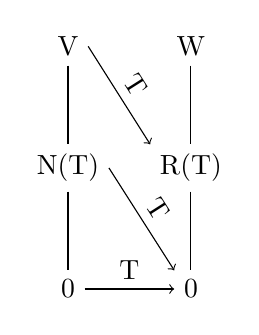
\begin{tikzpicture}
%Nodes
\node[]     (V)                     {V};
\node[]     (W)     [right=of V]    {W};
\node[]     (N)     [below=of V]    {N(T)};
\node[]     (R)     [below=of W]    {R(T)};
\node[]     (v0)    [below=of N]    {0};
\node[]     (w0)    [below=of R]    {0};

%Lines
\draw[-]    (V.south) -- (N.north);
\draw[-]    (W.south) -- (R.north);
\draw[->]   (V.east) -- (R.north west)
    node[midway, sloped, above]{T};
\draw[-]    (N.south) -- (v0.north);
\draw[-]    (R.south) -- (w0.north);
\draw[->]   (N.east) -- (w0.north west)
    node[midway, sloped, above]{T};
\draw[->]   (v0.east) -- (w0.west)
    node[midway, above]{T};
\end{tikzpicture}

\begin{proof}
$x \in V$는 $a_1,a_2, \cdots ,a_n \in F$에 대해서 $x=\sum_{i=1}^{n}{a_{i}v_{i}}$로 유일하게 표현할 수 있음.

선형변환 $T:\,V \rightarrow W$를 $T(v_i)=w_i$, $T(x)=\sum_{i=1}^{n}{a_{i}w_{i}}$라 정의하자.\footnote{이렇게 정의했을 때 해당 선형변환에 대해서 linear extension theorem이 성립하는지를 보는 것.}

(1) $T$는 선형인가?

$cT(v)+T(u)=T(cv+u)$가 성립함.

(2) $i=1,2, \cdots ,n$에 대하여 $T(v_i)=w_i$임.

(3) $T$는 유일한가?\footnote{정의한 $T(x)$가 유일한 선형변환임을 알 수 있음.}

선형변환 $U:\,V \rightarrow W$가 $i=1,2, \cdots ,n$에 대하여 $U(v_i)=w_i$를 만족한다고 가정하자. $x=\sum_{i=1}^{n}{a_{i}v_{i}} \in V$에 대해서, $U(x)=\sum_{i=1}^{n}{a_{i}w_{i}}=T(x)$이므로 $U=T$임.
\end{proof}

\textbf{Corollary}\, 두 벡터공간 $V,W$에 대하여 $V$가 유한집합인 기저 $\{v_1,v_2, \cdots ,v_n\}$를 포함한다고 가정하자. 두 선형변환 $U,T:\,V \rightarrow W$가 $i=1,2, \cdots ,n$일 때, $U(v_i)=T(v_i)$를 만족하면 $U=T$임.

즉, 기저에서 보낸 함숫값들의 조합이 같으면 같은 선형변환임.


\newpage


\part*{2. 선형변환의 행렬표현}

\section*{1. 순서기저(ordered basis)}

\subsubsection*{1) 정의}
유한차원 벡터공간 $V$의 순서기저(ordered basis)는 순서가 주어진 기저임. 즉, 순서기저는 일차독립이며 $V$를 생성하는 벡터들로 이루어진 수열임.

같은 벡터로 이루어져 있더라도 순서가 다르면 다른 순서기저임.

\subsubsection*{2) 표준 순서기저(standard ordered basis)}
벡터공간 $F^n$의 표준 순서기저는 $\{e_1,e_2, \cdots ,e_n\}$임.\\
$P_n(F)$의 표준 순서기저는 $\{1,x, \cdots ,x_n\}$임.\\
$R^n$의 표준 순서기저는 $\{{(1,0, \cdots), \cdots ,(\cdots ,0,1,0, \cdots), \cdots ,(\cdots ,0,1)}\}$


\section*{2. 좌표벡터(coordinate vector)}

\subsubsection*{1) 정의}
유한차원 벡터공간 $V$의 순서기저를 $\beta \{u_1,u_2, \cdots ,u_n\}$이라 하고, $x \in V$에 대해서 $a_1,a_2, \cdots ,a_n$은 $x = \sum_{i=1}^{n}{a_{i}u_{i}}$를 만족시키는 유일한 스칼라라 하자. $\beta$에 대한 좌표벡터(coordinate vector) $[x]_{\beta}$는 아래와 같음.

\[
[x]_{\beta} = 
\begin{pmatrix}
a_{1} \\
a_{2} \\
\vdots \\
a_{n}
\end{pmatrix}
\]

순서기저를 사용해 벡터를 $n$순서쌍으로 나타낸 것.\\
벡터를 좌표벡터로 표현하면 여러 계산에서 일종의 행렬로서 다룰 수 있게 됨.\\

\newpage


\section*{3. 선형변환의 행렬표현(matrix representation)}

선형변환을 행렬표현으로, 행렬표현으로 선형변환을 생각할 수 있음.

\subsubsection*{1) 정의\footnote{linear extension theorem이 이 정의가 가진 논리의 바탕이 됨.}}
유한차원 벡터공간 $V,W$와 각각의 순서기저 $\beta = \{v_1,v_2, \cdots ,v_n\}$, $\gamma = \{w_1,w_2, \cdots ,w_m\}$, 선형변환 $T:\,V \rightarrow W$가 있음. $j=1,2, \cdots ,n$일 때, $j$마다 다음을 만족하는 유일한 스칼라 $a_{ij} \in F$가 존재함.

\[
T(v_{j})=\sum_{i=1}^{m}{a_{ij}w_i}
\]

성분이 $A_{ij}=a_{ij}$인 $m \times n$ 행렬 $A$를 순서기저 $\beta$, $\gamma$에 대한 선형변환 $T$의 행렬표현(matrix representation)이라 하고, $A=[T]_{\beta}^{\gamma}$라 표기함. $V=W$, $\beta=\gamma$이면 간단히 $A=[T]_{\beta}$라 표기함.

선형변환 $T:\,V \rightarrow W$에 대해서 $V$의 기저의 함숫값을 $W$의 기저로 나타낸 것.

$j$번째 열은 $\gamma$에 대한 $T(v_j)$의 좌표벡터라고 볼 수 있음.

linear extension theorem의 Corollary에 의해, 선형변환 $U:\,V \rightarrow W$가 $[U]_{\beta}^{\gamma}=[T]_{\beta}^{\gamma}$를 만족하면 $U=T$임.


\subsubsection*{2) 영변환의 행렬표현}
$T_{0}(v_j)=0=0w_1+0w_2+ \cdots +0w_m$이므로 $[T_{0}]_{\beta}^{\gamma}=O$($m \times n$영행렬)임.

즉, 영변환의 행렬표현은 영행렬임.

\subsubsection*{3) 항등변환의 행렬표현\footnote{항등변환은 그 정의상 정의역과 공역이 동일한 벡터공간임.}}
$I_{v_j}=v_j=0v_1+0v_2+ \cdots +1v_j+ \cdots +0v_n$이므로 $I_V$의 $j$열은 $e_j$이고, $[I_{V}]_{\beta}^{\beta}=[I_{V}]_{\beta}$는 아래와 같음.

\[
[I_{V}]_{\beta}^{\beta}=[I_{V}]_{\beta}=
\begin{pmatrix}
1 & 0 & \cdots & 0\\
0 & 1 & \cdots & 0\\
\vdots & \vdots & & \vdots\\
0 & 0 & \cdots & 1
\end{pmatrix}
\]

즉, 항등변환의 행렬표현은 $n \times n$ 항등행렬임.\\


\newpage


\section*{4. 선형변환의 집합 $\mathcal{L}(V,W)$\footnote{새로운 집합과 함수가 등장했으므로, 지금까지 배운 내용을 생각해 보면 $\mathcal{L}(V,W)$가 벡터공간인지, $U(T)=[T]_{\beta}^{\gamma}$가 선형변환인지는 당연히 생각해봐야 하는 주제임.}}

\subsubsection*{1) 정의}
$F$-벡터공간 $V,W$에 대하여 $V$에서 $W$로 가는 모든 선형변환의 모임으로 이루어진 벡터공간을 $\mathcal{L}(V,W)$라 표기함. $V=W$이면 $\mathcal{L}(V,V)$를 간단히 $\mathcal{L}(V)$라 표기함.

Theorem 2.7에 의하면 $\mathcal{L}(V,W)$는 $F$-벡터공간임.

\subsubsection*{2) $[\cdot]_{\beta}^{\gamma}$는 선형변환인가?}
선형변환을 행렬표현으로 나타낼 수 있으므로, $T \in \mathcal{L}(V,W)$에 대해서 $U(T)=[T]_{\beta}^{\gamma}$인 $U:\mathcal{L}(V,W) \rightarrow M_{dim(W) \times dim(V)}(F)$라는 함수를 생각할 수 있음.

Theorem 2.8에 의하면 $U(T)=[T]_{\beta}^{\gamma}$는 선형변환임.

\subsubsection*{3) $\mathcal{L}(V,W)$의 기저}
$\mathcal{L}(V,W)$의 기저는 아래와 같음. (증명은 여종헌 프린트 참고.)

$$
T_{ij}(v_k)=\begin{cases}
    w_i\quad(k=j)\\
    0\,\,\quad(k \neq j)
\end{cases}
$$




\section*{5. 관련 정리}

\subsubsection*{1) $\mathcal{L}(V,W)$은 벡터공간인가?}
\textbf{Theorem 2.7}\, $F$-벡터공간 $V,W$와 선형변환 $T,U:V \rightarrow W$에 대하여 아래가 성립함.

먼저, 선형변환의 합과 스칼라 곱을 정의하자.\\
선형변환의 합과 스칼라 곱은 보편적인 함수의 집합($\mathcal{F}$)의 것과 같음.

\begin{enumerate}
    \item 임의의 $a \in F$에 대하여, $aT+U$는 선형임.
    \item 위 정의와 같이 선형변환의 합과 스칼라 곱을 정의할 때, $V$에서 $W$로 가는 모든 선형변환의 집합은 $F$-벡터공간임.
\end{enumerate}

선형변환의 집합($\mathcal{L}$)은 함수의 집합($\mathcal{F}$)의 부분공간임.

\begin{proof}
미리 정의한 함수의 합과 곱을 사용해 $(aT+U)(cx+y)=c(aT+U)(x)+(aT+U)(y)$임을 보이면 됨.

합과 곱에 대해서 닫혀 있고 $T_0$이 $\mathcal{L}(V,W)$에서 영벡터이므로 $\mathcal{L}(V,W)$는 벡터공간임.
\end{proof}


\subsubsection*{2) $U(T)=[T]_{\beta}^{\gamma}$는 선형변환인가?}
\textbf{Theorem 2.8}\, 유한집합 벡터공간 $V,W$와 각각의 순서기저 $\beta,\gamma$, 선형변환 $T,U:V \rightarrow W$에 대해서 아래가 성립함.

\begin{enumerate}
    \item $[T+U]_{\beta}^{\gamma}=[T]_{\beta}^{\gamma}+[U]_{\beta}^{\gamma}$
    \item 모든 스칼라 $a$에 대해서 $[aT]_{\beta}^{\gamma}=a[T]_{\beta}^{\gamma}$
\end{enumerate}

즉, $[\cdot]_{\beta}^{\gamma}$, 다시 말해 $U(T)=[T]_{\beta}^{\gamma}$는 선형변환임.

\begin{proof}
$\beta = \{v_1,v_2, \cdots ,v_n\}$, $\gamma = \{w_1,w_2, \cdots ,w_n\}$라 하자. $a_1, \cdots ,a_n, b_1, \cdots ,b_n \in F$, $j=1,2, \cdots ,n$에 대해서, $T(v_j)=\sum_{i=1}^{m}{a_{ij}w_i}$, $U(v_j)=\sum_{i=1}^{m}{b_{ij}w_i}$이고 $([T]_{\beta}^{\gamma})_{ij}=a_{ij}$, $([U]_{\beta}^{\gamma})_{ij}=b_{ij}$임. 이를 이용해 $(T+U)(v_j)$, $(aT)(v_j)$를 정리할 수 있음.
\end{proof}


\newpage


\part*{3. 선형변환의 합성과 행렬 곱}

\section*{1. 선형변환의 합성}

\subsubsection*{1) 새로운 연산의 필요성}
Theorem 2.9에 의하면 선형변환의 합성 또한 선형변환임.

지금까지 설명한 선형변환의 행렬표현은 선형변환의 합성에 대한 연산이 존재하지 않으므로 이를 정의해줘야 함.\\


\section*{2. 행렬 곱}

\subsubsection*{1) 정의}
$m \times n$ 행렬 $A$와 $n \times p$ 행렬 $B$에 대하여 두 행렬 $A,B$의 곱(product) $AB$는 아래와 같이 정의된 $m \times p$ 행렬임.

\[
1 \leq i \leq m,\,1 \leq j \leq p,\,(AB)_{ij}= \sum^{n}_{k=1}A_{ik}B_kj
\]

이 행렬 곱은 두 선형변환의 합성을 행렬로서 나타낸 연산임.

추가로, 곱셈의 소거법칙은 성립하지 않음.

\subsubsection*{2) 유도과정}
유한차원 벡터공간 $V,W,Z$와 선형변환 $T:V \rightarrow W$, $U:W \rightarrow Z$가 있음. $V$의 순서기저 $\{v_1, \cdots , v_n\}$, $W$의 순서기저 $\{w_1, \cdots , w_m\}$, $Z$의 순서기저 $\{z_1, \cdots , z_p\}$에 대하여 $A=[U]^{\gamma}_{\beta}$, $B=[T]^{\beta}_{\alpha}$라 하자.

$AB=[UT]^{\gamma}_{\alpha}$가 되도록 하는 행렬 곱을 정의할 것임. 선형변환의 행렬표현은 $T(v_{j})=\sum_{i=1}^{m}{a_{ij}w_i}$꼴에 의해 결정되므로, $(UT)(v_{j})$를 $\sum_{i=1}^{p}{C_{ij}z_i}$꼴로 나타내 $C_{ij}$에 대해 살펴볼 것임.

\begin{align*}
(UT)(v_j) &= U(T(v_j))=U(\sum_{k=1}^{m}{B_{kj}w_k})=\sum_{k=1}^{m}{B_{kj}}U(w_k)=\sum_{k=1}^{m}{B_{kj}}(\sum_{i=1}^{p}{A_{ik}z_i})=\sum_{i=1}^{p}{(\sum_{k=1}^{m}{A_{ik}B_{kj}})z_i}\\
&= \sum_{i=1}^{p}{C_{ij}z_i}\,(C_{ij}=\sum_{k=1}^{m}{A_{ik}B_{kj}})    
\end{align*}

즉, 성분이 $c_{ij}=C_{ij}$인 $q \times n$ 행렬 $c$는 선형변환 $UT$의 행렬표현 $[UT]_{\alpha}^{\gamma}$임.

여기서의 $C_{ij}=\sum_{k=1}^{m}{A_{ik}B_{kj}}$를 행렬 곱으로 정의함.

\subsubsection*{3) 행렬 곱과 행렬의 크기\footnote{이는 기저의 개수를 생각하면 당연함.}}
행렬 곱을 하는 두 행렬의 내부 차원이 같아야 행렬 곱이 정의됨.

행렬 곱을 하는 두 행렬의 외부 차원은 결과로 만들어지는 행렬의 크기를 결정함.

\subsubsection*{4) 연속적인 행렬 곱의 표현}
$n \times n$ 행렬 $A$에 대해서, $A^1=A,A^2=AA,A^3=A^2A, \cdots$로 정의함.
즉, 2 이상의 자연수 $k$에 대해서, $A^k=A^{k-1}A$라 정의함. 이때, $A^0=I_n$임.


\newpage


\section*{3. 선형변환의 합성과 행렬 곱 사이의 관계}
\subsubsection*{1) 대응관계}
행렬 곱의 유도과정과 Theorem 2.9에서 확인할 수 있듯이, 선형변환의 합성과 행렬 곱은 서로 완전히 대응됨.

\subsubsection*{2) 동일한 성질}
Theorem 2.10, 2.12, 2.16 등에서 확인할 수 있듯이, 선형변환의 합성과 행렬 곱은 아래의 성질들을 공유함.

\begin{enumerate}
    \item 분배법칙 성립.
    \item 결합법칙 성립.
    \item 항등원 성립. (항등변환, 항등행렬)
    \item 스칼라 곱의 분배법칙 성립.
    \item 교환법칙 성립하지 않음.\footnote{즉, $TU \neq UT$, $AB \neq BA$임}\\
\end{enumerate}


\section*{4. 좌측 곱 변환}

행렬로 선형변환의 성질을, 또는 선형변환으로 행렬의 성질을 유추할 때 가장 유용하게 사용할 수 있는 도구.

\subsubsection*{1) 정의}
$A$는 $m \times n$ 행렬이고, 성분은 체 $F$의 원소임. 아래의 선형변환을 간단히 $L_A$라 표기하자.

\[
L_A:F^n \rightarrow F^m,\, L_A(x)=Ax
\]

$L_A$를 좌측 곱 변환이라 함. 이때 $x$는 $F^n$의 열벡터이고, $Ax$는 $A$와 $x$의 행렬 곱임.

\subsubsection*{2) 성질}
Theorem 2.15에서 알 수 있듯이, 좌측 곱 변환은 선형이고 해당 Theorem에 서술한 여러 성질들을 가짐.

이 성질들을 이용해 행렬의 결합법칙을 증명할 수 있음.


\newpage


\section*{4. 관련 정리}

\subsubsection*{1) 선형변환의 합성은 선형변환인가?}
\textbf{Theorem 2.9}\, $F$-벡터공간 $V,W,Z$와 선형변환 $T:V \rightarrow W$, $U:W \rightarrow Z$를 생각하자. 두 선형변환의 합성 $UT:V \rightarrow Z$는 선형변환임.

\subsubsection*{2) 선형변환의 합성이 가지는 성질}
\textbf{Theorem 2.10}\, 벡터공간 $V$와 선형변환 $T,U_1,U_2 \in \mathcal{L}(V)$에 대해서 아래가 성립함.

\begin{enumerate}
    \item $T(U_1+U_2)=TU_1+TU_2$이고, $(U_1+U_2)T=U_1T+U_2T$ (분배법칙)
    \item $T(U_1U_2)=(TU_1)U_2$ (결합법칙\footnote{함수의 합성에서 결합법칙이 성립하는 것은 책의 부록에서 확인할 수 있음.})
    \item $TI=IT=T$
    \item 모든 스칼라 $a$에 대해서 $a(U_1U_2)=(aU_1)U_2=U_1(aU_2)$
\end{enumerate}

\subsubsection*{3) 선형변환의 합성과 행렬 곱}
\textbf{Theorem 2.11}\, 유한차원 벡터공간 $V,W,Z$와 각각의 순서기저 $\alpha,\beta,\gamma$, 선형변환 $T:V \rightarrow W$, $U:W \rightarrow Z$에 대해서 아래가 성립함.

\[
[UT]_{\alpha}^{\gamma}=[U]_{\beta}^{\gamma}[T]_{\alpha}^{\beta}
\]

행렬 곱의 유도과정과 정의를 생각하면 당연함.

\subsubsection*{4) 행렬 곱의 성질}
\textbf{Theorem 2.12}\, $A$가 $m \times n$ 행렬, $B$와 $C$가 $n \times p$ 행렬, $D$와 $E$가 $q \times m$ 행렬일 때, 다음이 성립함.

\begin{enumerate}
    \item $A(B+C)=AB+AC,\,(D+E)A=DA+EA$ (분배법칙)
    \item 임의의 스칼라 $a$에 대하여 $a(AB)=(aA)B=A(aB)$
    \item $I_{m}A=A=AI_{n}$
\end{enumerate}

이 성질은 각각 Theorem 2.10의 1, 4, 3과 대응됨.

\subsubsection*{5) 특정 열벡터 구하는 방법}
\textbf{Theorem 2.13}\, $m \times n$ 행렬 $A$와 $n \times p$ 행렬 $B$가 있음. $j=1,2, \cdots ,p$인 $j$에 대해서 $AB$의 $j$열을 $u_j$, $B$의 $j$열을 $v_j$라 표기하면 아래가 성립함.

\begin{enumerate}
    \item $u_j=Av_j$
    \item $v_j=Be_j$ (이때, $e_j$는 $F^p$의 $j$번째 표준 벡터\footnote{j번째만 1이고 나머지는 0인 tuple.})
\end{enumerate}

즉, AB의 특정 열벡터를 구하려면 A에다가 B의 (구하려는 순번의) 열벡터를 곱하면 됨.

B의 특정 열벡터를 구하려면 B 뒤에 $e_j$를 곱하면 됨.


\newpage


\subsubsection*{6) 좌표벡터의 행렬 곱}
\textbf{Theorem 2.14}\, $V,W$는 유한차원 벡터공간이고, 순서기저는 각각 $\beta, \gamma$임. 선형변환 $T:V \rightarrow W$와 $u \in V$에 대해서 아래가 성립함.

\[
[T(u)]_{\gamma}=[T]_{\beta}^{\gamma}[u]_{\beta}
\]

즉, 선형변환에 벡터를 대입하고 행렬로 표현하나, 선형변환의 행렬표현에 해당 벡터의 좌표벡터를 곱하나 동일함.

좌표벡터의 행렬 곱은 해당 선형변환에 대입하는 것과 같음.

\begin{proof}
$u \in V$를 고정하고 아래와 같은 선형변환 $f:F \rightarrow V,g:F \rightarrow W$를 정의하자.

\begin{center}
모든 $a \in F$에 대해서 $f(a)=au$, $g(a)=aT(u)$
\end{center}

$\alpha={1}$을 $F$의 표준 순서기저라 하자. $g =Tf$이므로 아래가 성립함.

\[
[T(u)]_{\gamma}=[g(1)]_{\gamma}=[g]_{\alpha}^{\gamma}=[Tf]_{\alpha}^{\gamma}=[T]_{\beta}^{\gamma}[f]_{\alpha}^{\beta}=[T]_{\beta}^{\gamma}[f(1)]_{\beta}=[T]_{\beta}^{\gamma}[u]_{\beta}
\]

\end{proof}

\subsubsection*{7) 좌측 곱 변환의 성질}
\textbf{Theorem 2.15}\, $A$는 $m \times n$ 행렬이고, 성분은 체 $F$의 원소임. 좌측 곱 변환 $L_A:F^n \rightarrow F^m$은 선형임.

또한 임의의 $m \times n$ 행렬 $B$(성분은 체 $F$의 원소)와 $F^n$의 표준 순서기저 $\beta$, $F^m$의 표준 순서기저 $\gamma$에 대해서 아래가 성립함.

\begin{enumerate}
    \item $[L_A]_{\beta}^{\gamma}=A$
    \item $L_A=L_B \Longleftrightarrow A=B$
    \item $L_{A+B}=L_A+L_B$
    \item 모든 $a \in F$에 대하여 $L_{aA}=aL_A$
    \item $T:F^n \rightarrow F^m$가 선형이면 $T=L_C$가 되도록 하는 $m \times n$ 행렬 $C$가 유일하게 존재함. $C=[T]_{\beta}^{\gamma}$임.
    \item $L_{AE}=L_{A}L_{E}$ ($E$는 $n \times p$ 행렬)
    \item $m=n$이면 $L_{I_n}=I_{F^n}$임.
\end{enumerate}

\begin{proof}
    (1) $[L_A]_{\beta}^{\gamma}$의 $j$열은 $L_A(e_j)$와 같음. $L_A(e_j)=Ae_j$는 $A$의 $j$열이므로 $[L_A]_{\beta}^{\gamma}=A$임.
    
    (2) $A=[L_A]_{\beta}^{\gamma}=[L_B]_{\beta}^{\gamma}=B$
    
    (5) 모든 $x \in F^n$에 대해서 $T(x)=Cx=L_C(x)$이므로 $T=L_C$임. 2번 성질에 의해 $C$는 유일함.
\end{proof}

\subsubsection*{8) 행렬 곱의 결합법칙}
\textbf{Theorem 2.16}\, 행렬 곱에서 결합법칙이 성립함. 즉, $A(BC)$를 정의할 수 있는 행렬 $A,B,C$는 $(AB)C$도 정의할 수 있고 $A(BC)=(AB)C$임.

이는 Theorem 2.10의 2와 대응됨. (선형변환의 합성의 결합법칙 성립과 대응됨.)

\begin{proof}
$L_{A(BC)}=L_{A}L_{BC}=L_{A}(L_{B}L_{C})=(L_{A}L_{B})L_{C}=L_{AB}L_{C}=L_{(AB)C}$

Theorem 2.15의 2번 성질에 의해 $A(BC)=(AB)C$임.
\end{proof}


\newpage


\part*{4. 가역성과 동형사상}

\section*{1. 함수의 역함수(inverse)와 가역(invertible)}

\subsubsection*{1) 정의}
벡터공간 $V,W$와 선형변환 $T:V \rightarrow W$를 생각하자. $TU=I_W$이고 $UT=I_V$인 함수 $U$를 $T$의 역함수(inverse)라 함. 이 역함수는 $T^{-1}$로 표기함.

역함수가 존재하는지를 가역(invertible)이라 함.

\subsubsection*{2) 성질}
함수가 가역이기 위한 필요충분조건은 해당 함수가 단사(injection)이고 전사(subjection)인 것임.

$T$가 가역이면 $T$의 역함수는 유일함.

$T^{-1}$은 가역임.

$(TU)^{-1}=U^{-1}T^{-1}$

$(T^{-1})^{-1}=T$임.

\subsubsection*{3) 역함수(inverse)의 선형성}
Theorem 2.17에 의하면 선형변환의 역함수 또한 선형변환임.\\


\section*{2. 행렬의 역행렬(inverse)과 가역(invertible)}
\subsubsection*{1) 정의}
$n \times n$ 행렬 $A$에 대해서 $AB=BA=I$인 $n \times n$ 행렬 $B$를 $A$의 역행렬(inverse)이라고 함. 이 역행렬은 $A^{-1}$로 표기함.

역행렬이 존재하는지를 가역(invertible)이라고 함.

정의에서 알 수 있듯이, 정사각행렬(정방행렬)이 아니면 가역일 수 없음.

\subsubsection*{2) 성질}
$A$가 가역이면 $A$의 역행렬은 유일함.

\subsubsection*{3) 구하는 방법}

행렬의 역행렬을 구하는 방법은 3절에서 다룸.


\newpage


\section*{3. 동형(isomorphic)과 동형사상(isomorphism)}
구체적으로는 다르지만 구조적으로는 같은 것을 동형(isomorphic)이라 함.

\subsubsection*{1) 정의}
두 벡터공간 $V,W$ 사이에 가역인 선형변환 $T:V \rightarrow W$가 존재하면 $V$와 $W$는 동형(isomorphic)임. 이때 가역인 선형변환을 $V$에서 $W$로 가는 동형사상(isomorphism)이라 함.

무엇이 무엇과 동형이라는 개념은 동치관계임. 즉, $V$는 $V$와 동형이고, $V$가 $W$와 동형이면 $W$가 $V$와 동형이고, $V$가 $W$와 동형이고 $W$가 $S$와 동형이면 $V$가 $S$와 동형임.\\
간단히 정리하면 '그저 $V$와 $W$는 동형'인 것.

\subsubsection*{2) 동형이기 위한 필요충분조건}
Theorem 2.19에 의하면, 같은 체 위의 두 벡터공간의 차원이 같다면 두 벡터공간은 동형임.

즉, 차원이 같음 = 동형임 = 가역인 선형변환이 존재함.

\subsubsection*{3) 동형사상과 '이름 바꾸기'}
동형사상은 구조적으로 동일한 두 벡터공간을 이어준다는 점에서 벡터공간의 '이름만 바꾸는' 기능을 한다고 이해할 수 있음.

일례로, 선형변환의 행렬표현이 가능했던 것 또한 사실 선형변환의 집합과 행렬의 집합이 동형이고, $[]_{\beta}^{\gamma}$가 '선형변환의 이름을 행렬로 바꾸는' 동형사상이기 때문임.\\

아래의 그림은 벡터공간 $V,W$에 대해 동형사상(isomorphism) $T:V \rightarrow W$이 어떤 식으로 '이름을 바꾸는지'를 나타낸 다이어그램임. $V$의 연산을 $W$의 연산으로 바꾸고 있음.

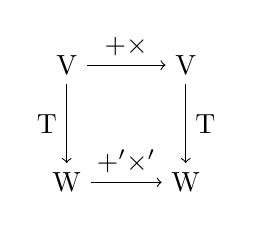
\begin{tikzpicture}
%Nodes
\node[]     (V1)                    {V};
\node[]     (V2)    [right=of V1]   {V};
\node[]     (W1)    [below=of V1]   {W};
\node[]     (W2)    [below=of V2]   {W};

%Lines
\draw[->]   (V1.east) -- (V2.west)
    node[midway, above]{$+ \times$};
\draw[->]   (W1.east) -- (W2.west)
    node[midway, above]{$+^{\prime} \times^{\prime}$};
\draw[->]   (V1.south) -- (W1.north)
    node[midway, left]{T};
\draw[->]   (V2.south) -- (W2.north)
    node[midway, right]{T};
\end{tikzpicture}


\section*{4. 표준표현(standard representation)}
\subsubsection*{1) 정의}
체 $F$에서의 $n$차원 벡터공간 $V$의 순서기저를 $\beta$라 하자. $\beta$에 대한 $V$의 표준표현(standard representation)은 아래와 같이 정의된 함수 $\phi_{\beta}:V \rightarrow F^n$임.

\[
x \in V,\,\phi_{\beta}(x)=[x]_{\beta}
\]

즉, 벡터를 좌표벡터로 나타내는 함수.

\subsubsection*{2) 선형성과 동형성}
$\phi_{\beta}$는 선형변환임.

Theorem 2.21에 의하면 $\phi_{\beta}$는 벡터공간 $V$와 그 순서기저 $\beta$에 대해서 동형사상임.\\
이는 곧 $n$차원 벡터공간과 $F^n$이 동형이라는 것을 의미함.


\newpage


\subsubsection*{3) 선형변환 합성의 가환적 그래프}
차원이 각각 $n,m$인 벡터공간 $V,W$와 각각의 순서기저 $\beta, \gamma$, 선형변환 $T:V \rightarrow W$가 있다고 하자. $\phi_{\beta}$를 이용하면 $V$와 $F^n$을 동일시할 수 있고, $\phi_{\gamma}$를 이용하면 $W$와 $F^m$을 동일시할 수 있음. 즉, $T$와 $L_{[T]_{\beta}^{\gamma}}$또한 동일시할 수 있음. 이를 아래와 같이 수식으로 나타낼 수 있음.

\[
L_{[T]_{\beta}^{\gamma}}\phi_{\beta}=\phi_{\gamma}T
\]

이것을 이용하면 임의의 두 벡터공간 사이에 정의된 연산을 $F^n$과 $F^m$ 사이에 정의된 연산으로 나타낼 수 있음.

\begin{figure}[hbt!]
    \centering
    \includegraphics[width=5cm, height=5cm]{images/2.4.png}\\
\end{figure}

\section*{5. 관련 정리}
\subsubsection*{1) 역함수의 선형성}
\textbf{Theorem 2.17}\, 벡터공간 $V,W$와 가역인 선형변환 $T:V \rightarrow W$에 대해서 역함수 $T^{-1}:V \rightarrow W$ 또한 선형임.

\textbf{Corollary}\, 선형변환 $T:V \rightarrow W$가 가역이라고 하자. $V$가 유한차원이기 위한 필요충분조건은 $W$가 유한차원인 것임. 특히 이때 $dim(V)=dim(W)$임.

즉, 가역인 선형변환이 존재하면 두 벡터공간 모두가 유한차원이거나 무한차원이고, 유한차원인 경우 두 벡터공간의 차원도 같음.

\subsubsection*{2) 선형변환의 역함수와 행렬의 역행렬의 관계}
\textbf{Theorem 2.18}\, 유한차원 벡터공간 $V,W$와 각각의 순서기저 $\beta,\gamma$, 선형변환 $T:V \rightarrow W$에 대해서 $T$가 가역이기 위한 필요충분조건은 $[T]^{\gamma}_{\beta}$가 가역인 것임. 특히, $[T^{-1}]_{\gamma}^{\beta}=([T]_{\beta}^{\gamma})^{-1}$임.

이를 도식으로(항상 나오는 사각형의 그림.) 생각해 보면 이해가 편함.

\textbf{Corollary}\, $n \times n$ 행렬 $A$가 가역이기 위한 필요충분조건은 $L_A$가 가역인 것임. 특히, $(L_A)^{-1}=L_{A^{-1}}$임.

\subsubsection*{3) 동형이기 위한 필요충분조건}
\textbf{Theorem 2.19}\, 같은 체 위에서 정의된 유한차원 벡터공간 $V,W$에 대해서 $V$와 $W$가 동형이기 위한 필요충분조건은 $dim(V)=dim(W)$임.

\begin{proof}
1. $V,W$가 동형임. $\cdots$ $dim(V)=dim(W)$
$V,W$는 가역인 선형변환이 존재하고 유한차원이므로, Theorem 2.17의 Corollary에 의해 $dim(V)=dim(W)$임.

2. $dim(V)=dim(W)$ $\cdots$ $V,W$가 동형임.
$dim(V)=dim(W)=n$, $V$의 기저를 $\alpha=\{v_1, \cdots ,v_n\}$, $W$의 기저를 $\beta=\{w_1, \cdots ,w_n\}$라 하자. linear extension theorem에 의하면 $T(v_i)=w_i\,(1 \leq i \leq n)$인 선형변환 $T:V \rightarrow W$가 존재함. $R(T)=span(T(\alpha))=span(\beta)=W$이므로 $T$는 전사(onto, subjection)임. Theorem 2.5에 의해 $T$는 단사이므로 동형사상임.
\end{proof}


\newpage


\subsubsection*{4) $\Phi^{\gamma}_{\beta}$의 동형성}
\textbf{Theorem 2.20}\, 차원이 각각 $n,m$인 $F$-벡터공간 $V,W$를 생각하자. $V,W$의 순서기저를 각각 $\beta,\gamma$라 할 때, 아래와 같이 정의한 함수 $\Phi^{\gamma}_{\beta}:\mathcal{L}(V,W) \rightarrow M_{m \times n}(F)$는 동형사상임.

\[
T \in \mathcal{L}(V,W),\,\Phi^{\gamma}_{\beta}=[T]^{\gamma}_{\beta}
\]

즉, 선형변환의 집합과 행렬의 집합은 동형이고, 선형변환의 행렬표현을 나타내는 $[]_{\beta}^{\gamma}$는 동형사상임.\\
이를 Fundamental Theorem of Linear Algebra라고 함. (선형사상=행렬)

\begin{proof}
동형사상은 가역인 선형변환임. Theorem 2.8에 의하면 $\Phi^{\gamma}_{\beta}$는 선형이므로 전단사인 것을 보여야 함. 임의의 $m \times n$ 행렬 $A$에 대해서 $\Phi^{\gamma}_{\beta}(T)=A$인 선형변환 $T:V \rightarrow W$가 유일하게 존재함을 보이면 됨.

$\beta=\{v_1, \cdots ,c_n\}$, $\gamma=\{w_1, \cdots ,w_m\}$이라 하면, linear extension theorem에 의해 아래와 같이 정의된 선형변환 $T:V \rightarrow W$가 유일함.

\[
T(v_j)=\sum_{i=1}^{m}A_{ij}w_i\,(1 \leq j \leq n)
\]

즉, 행렬 $A$에 대해 선형변환 $T$가 유일함.

+ 여종헌 프린트에 $\mathcal{L}(V,W)$의 차원을 직접 구해 증명하는 방법도 나와있음.
\end{proof}

\textbf{Corollary}\, 차원이 각각 $n,m$인 유한차원 벡터공간 $V,W$에 대해서 $\mathcal{L}(V,W)$는 차원이 $nm$인 벡터공간임.

\subsubsection*{5) $\phi_{\beta}$의 동형성}
\textbf{Theorem 2.21}\, 임의의 유한차원 벡터공간 $V$와 순서기저 $\beta$에 대해서 $\phi_{\beta}$는 동형사상임.


\newpage

\part*{5. 좌표변환 행렬}

\section*{1. 좌표변환 행렬(change of coordinate matrix)}

\subsubsection*{1) 정의}
Theorem 2.22에 의하면, 유한차원 벡터공간 $V$의 두 순서기저 $\beta, \beta^{\prime}$에 대해서, $Q=[I_V]^{\beta}_{\beta^{\prime}}$라 하자. 아래가 성립함.

\begin{enumerate}
    \item $Q$는 가역행렬임.
    \item 임의의 $v \in V$에 대해서 $[v]_{\beta}=Q[v]_{\beta^{\prime}}$
\end{enumerate}

즉, 좌표변환 행렬은 벡터공간의 어떤 벡터에 대해서, 특정 기저로 표현한 좌표벡터를 다른 기저로 표현한 좌표벡터로 만들 수 있는 것.

$Q$는 $\beta^{\prime}$좌표를 $\beta$좌표로 변환한다고 함.

이때, $Q^{-1}$은 $\beta$좌표를 $\beta^{\prime}$좌표로 변환함.\\


\section*{2. 선형변환 행렬표현의 전환}
\subsubsection*{1) 선형변환 행렬표현의 전환}
Theorem 2.23에 의하면, 한 선형변환의 행렬표현을 다른 기저를 이용한 동일한 선형변환의 행렬표현으로 전환할 수 있음. 아래가 그 식임. 이때 $Q$는 $\beta^{\prime}$좌표를 $\beta$좌표로 옮기는 좌표변환 행렬임.

\begin{center}
$[T]_{\beta^{\prime}}=[I_V]_{\beta}^{\beta^\prime}[T]^{\beta}_{\beta}[I_V]_{\beta^{\prime}}^{\beta}=Q^{-1}[T]_{\beta}Q$
\end{center}

\begin{center}
$[T]_{\alpha}^{\beta}=[I_W]_{\beta^\prime}^{\beta}[T]_{\alpha^{\prime}}^{\beta^{\prime}}[I_V]_{\alpha}^{\alpha^{\prime}}$\\
\end{center}

이때, 아래의 식 또한 성립함.

\[
[T]_{\beta}=[I_V]^{\beta}_{\beta^\prime}[T]^{\beta^{\prime}}_{\beta^{\prime}}[I_V]^{\beta^{\prime}}_{\beta}=Q[T]_{\beta^{\prime}}Q^{-1}
\]

\section*{3. 닮음(similar)\footnote{닮음에 대한 자세한 이야기는 5~7장에서 다룸.}}
\subsubsection*{1) 정의}
$A,B$가 $M_{n \times n}(F)$의 행렬이라 하자. $B=Q^{-1}AQ$인 가역행렬 $Q$가 존재하면 $B$는 $A$와 서로 닮음(similar)임.

즉, 동일한 선형변환에 대해 서로 다른 두 행렬표현은 서로 닮은(similar)임.

닮음 관계는 동치관계임.


\newpage


\section*{4. 관련 정리}
\subsubsection*{1) 좌표변환 행렬(change of coordinate matrix)의 정의}
\textbf{Theorem 2.22}\, 유한차원 벡터공간 $V$의 두 순서기저 $\beta, \beta^{\prime}$에 대해서, $Q=[I_V]^{\beta}_{\beta^{\prime}}$라 하자. 아래가 성립함.

\begin{enumerate}
    \item $Q$는 가역행렬임.
    \item 임의의 $v \in V$에 대해서 $[v]_{\beta}=Q[v]_{\beta^{\prime}}$
\end{enumerate}

$Q$는 $\beta^{\prime}$좌표를 $\beta$좌표로 변환한다고 함.

\begin{proof}
1. $Q=[I_V]^{\beta}_{\beta^{\prime}}$인데, $I_V$가 가역이므로, $Q$ 또한 가역임.

2. $[v]_{\beta}=[I_V(v)]_{\beta}=[I_V]_{\beta^{\prime}}^{\beta}[v]_{\beta^{\prime}}=Q[v]_{\beta^{\prime}}$
\end{proof}

\subsubsection*{2) 선형변환 행렬표현의 전환}
\textbf{Theorem 2.23}\, 유한차원 벡터공간 $V$의 선형연산자 $T$와 $V$의 순서기저 $\beta$, $\beta^{\prime}$이 있음. $Q$가 $\beta^{\prime}$좌표를 $\beta$좌표로 옮기는 좌표변환 행렬이라 하면 아래가 성립함.

\[
[T]_{\beta^{\prime}}=[I_V]_{\beta}^{\beta^\prime}[T]^{\beta}_{\beta}[I_V]_{\beta^{\prime}}^{\beta}=Q^{-1}[T]_{\beta}Q
\]

즉, $T$가 유한차원 벡터공간 $V$의 선형연산자이고 $\beta$와 $\beta^{\prime}$이 $V$의 순서기저일 때, $[T]_{\beta^{\prime}}$과 $[T]_{\beta}$는 서로 닮음(similar)임.

이를 더 일반화하여 $V,W$ 사이에 정의된 선형변환 $T:V \rightarrow W$에 대해 나타내면 아래와 같음.

\[
[T]_{\alpha}^{\beta}=[I_W]_{\beta^\prime}^{\beta}[T]_{\alpha^{\prime}}^{\beta^{\prime}}[I_V]_{\alpha}^{\alpha^{\prime}}
\]

\begin{proof}
방법1. 선형변환 행렬표현의 전환을 함수의 합성으로 나타내기.

벡터공간 $V$의 기저 $\alpha, \alpha^{\prime}$와 $W$의 기저 $\beta, \beta^{\prime}$에 대해서, 벡터의 이동을 고려하면 아래의 다이어그램을 생각할 수 있음. 즉, $[T]_{\alpha}^{\beta}=[I_W]_{\beta^\prime}^{\beta}[T]_{\alpha^{\prime}}^{\beta^{\prime}}[I_V]_{\alpha}^{\alpha^{\prime}}$임. $W$ 대신 $V$를 넣으면 위 식을 유도할 수 있음.

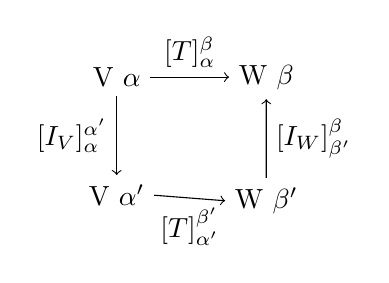
\begin{tikzpicture}[scale=10]
%Nodes
\node[]     (V1)                    {V $\alpha$};
\node[]     (V2)    [below=of V1]   {V $\alpha^{\prime}$};
\node[]     (W1)    [right=of V1]   {W $\beta$};
\node[]     (W2)    [below=of W1]   {W $\beta^{\prime}$};

%Lines
\draw[->]   (V1.south) -- (V2.north)
    node[midway, left]{$[I_V]_{\alpha}^{\alpha^{\prime}}$};

\draw[->]   (W2.north) -- (W1.south)
    node[midway, right]{$[I_W]_{\beta^{\prime}}^{\beta}$};

\draw[->]   (V1.east) -- (W1.west)
    node[midway, above]{$[T]_{\alpha}^{\beta}$};
    
\draw[->]   (V2.east) -- (W2.west)
    node[midway, below]{$[T]_{\alpha^{\prime}}^{\beta^{\prime}}$};
\end{tikzpicture}

방법2. 단순 유도하기.

$Q[T]_{\beta^{\prime}}=[I]_{\beta^{\prime}}^{\beta}[T]_{\beta^{\prime}}^{\beta^{\prime}}=[IT]_{\beta^{\prime}}^{\beta}=[TI]_{\beta^{\prime}}^{\beta}=[T]_{\beta}^{\beta}[I]_{\beta^{\prime}}^{\beta}=[T]_{\beta}Q$
\end{proof}

\textbf{Corollary}\, $A \in M_{n \times n}(F)$와 $F^n$의 순서기저 $\gamma$에 대해서 아래가 성립함.

\[
[L_A]_{\gamma}=Q^{-1}AQ
\]

이때, $n \times n$ 행렬 $Q$의 $j$열은 $\gamma$의 $j$번째 벡터임.


\newpage

%3.기본행렬연산과 연립일차방정식
\part{\textit{\underline{기본행렬연산과 연립일차방정식}}}
\part*{1. 기본행렬연산과 기본행렬}

\section*{1. 기본연산(elementary operation)}

\subsubsection*{1) 정의}
$m \times n$ 행렬 $A$에 대해서 $A$의 행[열]에 대한 아래의 세 연산을 기본행[열]연산(elementary row[column] operation)이라 함.

\begin{enumerate}
    \item $A$의 두 행[열]을 교환하는 것.
    \item $A$의 한 행[열]에 영이 아닌 스칼라를 곱하는 것.
    \item $A$의 한 행[열]에 다른 행[열]의 스칼라 배를 더하는 것.
\end{enumerate}

행연산(row operation)과 열연산(column operation)을 통틀어 기본연산(elementary operation)이라 함.

기본연산의 1, 2, 3을 각각 1형(type), 2형, 3형이라 함.\\


\section*{2. 기본행렬(elementary matrix)}

\subsubsection*{1) 정의}
$n \times n$ 기본행렬(elementary matrix)은 항등행렬 $I_n$에 기본연산을 한 번 적용하여 얻은 행렬임.

$I_n$에 1형, 2형, 3형 연산을 하여 얻은 행렬을 각각 1형, 2형, 3형이라고 함.

\subsubsection*{2) 기본연산의 적용}
Theorem 3.1에 의하면, 기본연산을 적용하는 것은 그 행렬에 적절한 기본행렬을 곱하는 것과 같음.

이 덕분에 기본연산을 적용하는 것을 수식적으로 나타낼 수 있음.


\newpage


\section*{3. 관련 정리}
\subsubsection*{1) 기본연산과 기본행렬의 곱}
\textbf{Theorem 3.1}\, 행렬 $A \in M_{m \times n}(F)$에 기본행[열]연산을 하여 행렬 $B$를 얻었다면, $B=EA[B=AE]$가 되는 $m \times m[n \times n]$ 기본행렬 $E$가 존재함. 이때, $A$에서 $B$를 얻은 기본행[열]연산을 $I_m[I_n]$에 똑같이 적용하면 행렬 $E$가 됨. 역으로 $E$가 $m \times m[n \times n]$ 기본행렬일 때, $I_m[I_n]$에서 $E$를 얻은 기본행[열]연산을 $A$에 똑같이 적용하면 $EA[AE]$가 됨.

즉, 기본행렬을 곱하는 것은 그 기본행렬에 해당하는 기본연산을 적용하는 것과 같음.

\subsubsection*{2) 기본행렬의 가역성}
\textbf{Theorem 3.2}\, 기본행렬은 가역임. 그 역행렬은 같은 종류의 기본행렬임.

\begin{proof}
기본행렬을 만든 연산을 거꾸로 수행하면(해당하는 기본행렬 곱하면) 항등행렬이 나오므로 기본행렬은 가역임.\\
\end{proof}


\section*{4. 기본행연산으로 역행렬 구하기}

\subsubsection*{1) }


\newpage


\part*{2. 행렬의 랭크}

\section*{1. 행렬의 랭크}
\subsubsection*{1) 정의}
행렬 $A \in M_{m \times n}(F)$에 대해서 $A$의 랭크(rank)는 선형변환 $L_A:F^n \rightarrow F^m$의 랭크로 정의하고 $rank(A)$라 표기함.

\subsubsection*{2) 행렬의 랭크와 가역성}
\begin{center}
$n \times n$ 행렬이 가역이기 위한 필요충분조건은 행렬의 랭크가 $n$인 것임.    
\end{center}

\begin{proof}
1. $n \times n$ 행렬 $A$가 가역 $\rightarrow$ 행렬 $A$의 랭크가 $n$.
Theorem 2.18의 Corollary에 의해, $A$가 가역이면 $L_A$도 가역임. 즉 $dim(F^n)=rank(L_A)=n$임. $L_A$의 랭크가 행렬 $A$의 랭크이므로 성립.

2. 행렬 $A$의 랭크가 $n$ $\rightarrow$ $n \times n$ 행렬 $A$가 가역.
$rank(L_A)=dim(F^n)$이고, $L_A:F^n \rightarrow F^n$으로 정의역과 공역의 차원이 같으므로 행렬 $A$는 가역임.
\end{proof}

\subsubsection*{3) 행렬의 랭크와 선형변환의 랭크}
Theorem 3.3에 의하면, 선형변환의 랭크와 그 행렬표현의 랭크는 동일함.

그러므로, 선형변환의 랭크를 찾는 문제는 그 행렬표현의 랭크를 찾는 문제와 귀결됨.\\


\section*{2. 행렬의 랭크 구하기}
\subsubsection*{1) 행렬의 랭크를 보존하는 연산}
Theorem 3.4에 의하면, 가역행렬의 곱은 행렬의 랭크를 보존하는 연산임.

Theorem 3.4의 Corollary에 의해, 행렬의 기본연산은 랭크를 보존함.\\
즉, 행렬에 기본연산을 적용하여(기본행렬을 곱하여) 랭크를 구하기 더 쉬운 형태로 바꿀 수 있음.

\subsubsection*{2) 행렬의 랭크 구하기}
Theorem 3.5에 의하면, 임의의 행렬의 랭크는 일차독립인 열의 최대 개수임.

즉, 행렬의 랭크는 아래의 방법으로 구할 수 있음.
\begin{enumerate}
    \item 기본연산으로 행렬을 정리함.
    \item 일차독립인 열의 개수를 확인함.
\end{enumerate}

이에 대한 구체적 방법은 Theorem 3.6에서 확인할 수 있는데, 행렬에 기본연산을 유한 번 사용해 왼쪽 위가 $I_r$이고 나머지는 0인 행렬로 만들 수 있다는 것. 이 꼴로 만들면 일차독립인지를 확인하는 것이 굉장히 간단해짐.


\section*{3. 관련 정리}
\subsubsection*{1) 행렬의 랭크과 선형변환의 랭크}
\textbf{Theorem 3.3}\, 유한차원 벡터공간 사이에서 정의된 선형변환 $T:V \rightarrow W$와 $V,W$ 각각의 순서기저 $\beta, \gamma$에 대해서 $rank(T)=rank([T]^{\gamma}_{\beta})$임.

즉, 선형변환의 랭크과 그 행렬표현의 랭크는 동일함.

\subsubsection*{2) 행렬의 랭크를 보존하는 연산}
\textbf{Theorem 3.4}\, $m \times n$ 행렬 $A$, $m \times m$ 가역행렬 $P$, $n \times n$ 가역행렬 $Q$에 대해서 아래가 성립함.

\begin{enumerate}
    \item $rank(AQ)=rank(A)$
    \item $rank(PA)=rank(A)$
    \item $rank(PAQ)=rank(A)$
\end{enumerate}

즉, 가역행렬의 곱은 행렬의 랭크를 보존하는 연산임.

\textbf{Corollary}\, 행렬의 기본행연산과 기본열연산은 랭크를 보존함.

\begin{proof}
기본연산은 기본행렬을 곱하는 것인데, 기본행렬은 정사각행렬인 가역행렬이므로 행렬의 랭크를 보존함.
\end{proof}

\subsubsection*{3) 행렬의 랭크}
\textbf{Theorem 3.5}\, 임의의 행렬의 랭크는 일차독립인 열의 최대 개수와 같음. 즉, 행렬의 랭크는 그 열에 의해 생성된 부분공간의 차원임.

즉, 행렬의 각 열을 하나의 벡터로 생각했을 때, 일차독립인 열들의 집합을 만들면 그 개수가 곧 랭크임.

행렬의 열은 곧 기저를 보낸 것을 의미하는데, 상공간 생성 방법을 생각해 보면 이 정리는 매우 당연함.

\subsubsection*{4) 행렬의 랭크를 구하는 구체적 방법}
\textbf{Theorem 3.6}\, 랭크가 $r$인 $m \times n$ 행렬 $A$를 생각하자. $r \leq m,\,r \leq n$이 성립하고 기본행연산과 기본열연산을 유한 번 사용하여 $A$를 아래와 같은 꼴로 바꿀 수 있음.
\[
D=
\begin{pmatrix}
I_r & O_1\\
O_2 & O_3
\end{pmatrix}
\]

이때, $i \leq r$이면 $D_{ii}=1$, 그렇지 않으면 $D_{ij}=0$이고 $O_1,\,O_2,\,O_3$은 영행렬임.

즉, 행렬에 기본연산을 유한 번 사용해 왼쪽 위가 $I_r$이고 나머지는 0인 행렬로 만들 수 있음.

증명은 프리드버그 p.179에 있지만 굳이 정리하지 않겠음.

\textbf{Corollary 1}\, Theorem 3.5의 행렬 $A$에 대해서, $D=BAC$를 만족하는 $m \times m$ 가역행렬 $B$, $n \times n$ 가역행렬 $C$가 존재함.

즉, 행렬에 기본행렬을 곱해 $D$로 만들 수 있다는 것.

\textbf{Corollary 2}\, $m \times n$ 행렬에 대해 아래가 성립함.
\begin{enumerate}
    \item $rank(A^t)=rank(A)$
    \item 임의의 행렬의 랭크는 일차독립인 행의 최대 개수와 같음. 행렬의 랭크는 그 행에 의해 생성된 부분공간의 차원임.
    \item 임의의 행렬의 행과 열은 차원이 같은 부분공간을 생성함. 각각의 차원은 행렬의 랭크와 같음.
\end{enumerate}

\begin{proof}
(1) Corollary 1에 의하면 $D=BAC$인데, $D^t=(BAC)^t=C^{t}A^{t}B^{t}$임. $C^{t}$, $B^{t}$는 가역이므로 $rank(C^{t}A^{t}B^{t})=rank(A^{t})=rank(D^t)$인데, $rank(D^t)=rank(D)=rank(A)$임.

(2) 전치해 보면 확인할 수 있음.

(3) Theorem 3.5, Theorem 3.6의 Corollary 2 (1), (2)를 보면 알 수 있음.
\end{proof}

\textbf{Corollary 3}\, 모든 가역행렬은 기본행렬의 곱으로 나타남.

\begin{proof}
$n \times n$ 가역행렬 $A$의 랭크는 $n$임. $D=I_n=BAC$임. $B$와 $C$는 각각 $B=E_{p}E_{p-1} \cdots E_{1}$, $C=G_{1}G_{2} \cdots G_{q}$를 만족하는 기본행렬 $E_{i},\,G_{i}$가 존재함. 정리하면 아래와 같음.

\[
A=B^{-1}I_{n}C^{-1}=B^{-1}C^{-1}=E_{1}E_{2} \cdots E_{p}G_{q}G_{q-1} \cdots G_{1}
\]

즉, 행렬 $A$는 기본행렬의 곱으로 나타낼 수 있음.
\end{proof}

\newpage


\end{document}
